% --
% training details

\section{Implementation and Experiment Details}\label{sec:exp_details}
The implementation describes the used software tools for the experiments on the neural networks, such as the programming language and packages for the source code.
The training details provide commonly used sets of hyperparameters applied to train neural networks.
Note that the training details can vary between different experiments and models and that the listing provide an overview of all available parameters to choose from with recommendations of parameters for the speech command dataset.
If parameters are varying in some experiments, they are usually noted, otherwise the parameters listed were used.
The evaluation details of the models is described separately and evaluates the trained models upon accuracy performance, and noise and shift invariance.


% --
% implementation notes

\subsection{Implementation Notes}\label{sec:exp_details_implementation}
The source code for this thesis was entirely written in \texttt{Python} with version $>3.8$ evaluated on a Linux operating system and is open source available at \cite{KWSGame}.
The operating system might be relevant, if someone tries to run the python code on a \enquote{Windows} machine, where unexpected errors might occur (especially regarding path variables).
Also the project does not download the speech command dataset by its own and a path to the dataset has to be specified in the \texttt{config.yaml} file of the project.
More information about how to run the project is described in the \texttt{README.txt} file of the project.
The training and implementation of all used neural networks were done with the \texttt{Pytorch} \cite{Pytorch} framework of version $1.7.0$. 
Usually it should not be a problem if a newer version of \texttt{Pytorch} is used, during the work on the thesis the version changed to $1.9.0$ without any version depending problems.
The feature extraction of MFCCs was self implemented but uses already existing and efficient code for signal transformations, such as the STFT or DCT, with packages from \texttt{Scipy}.
All matrix-vector computations were done with the well known package \texttt{Numpy} or with \texttt{Pytorch}.
Several other \texttt{Python} packages were used within the project but are not named explicitly.
They can be looked up in the open source repository of the project, if requested.


% --
% training details

\subsection{Neural Network Training Details}\label{sec:exp_details_training}
The training details and parameters of the used neural networks can be split into following components: Feature extraction, dataset, training, and pre-training.
The feature extraction parameters provide information about the extraction of MFCC features.
The dataset parameters are the selected labels and the number of examples per labels for training.
To specify the training of neural networks, the training hyperparameters, such as the learning rate or batch size, are applied.
Further, the pre-training details describe a separate training of GANs to use the obtained weights for transfer learning on an equivalent CNN.


% --
% feature

\subsubsection{Feature Extraction Parameters}
During the feature selection experiments in \rsec{exp_fs}, the feature extraction parameters for cepstral coefficients with enhancements were varying.
If not other stated, the feature extraction parameters in \rtab{exp_details_params_feature} were used.
% --
% feature extraction parameters
\begin{table}[ht!]
\begin{center}
\caption{Parameters for MFCC feature extraction.}
\begin{tabular}{ M{6cm}  M{2cm} M{2cm}}
\toprule
\textbf{Parameter} & \textbf{Value} & \textbf{Varying for experiments} \\
\midrule
Speech signal length & \SI{500}{\milli\second} & - \\
Analytic window size & \SI{25}{\milli\second} & -\\
Hop size & \SI{10}{\milli\second} & -\\
Window Function & Hanning & -\\
\midrule
Number of filter bands & 32 & -\\
Number of cepstral coefficients & 12 & yes\\
Delta features & no & yes \\
Double delta features & no & yes \\
Energy features & no 	& yes \\
Frame based normalization & yes & yes\\
\bottomrule
\label{tab:exp_details_params_feature}
\end{tabular}
\end{center}
\end{table}
\FloatBarrier
\noindent


% --
% dataset

\subsubsection{Dataset Parameters}
The labels for training are selected to the same 12 labels (L12) that were also used in the benchmark networks, described in \rsec{prev_kws_benchmark}, to provide a comparison for the performed experiments in this section and the previous work.

The maximum number of examples per label for training is given by the minimum examples per selected label for each label and each set.
This is provided by the validation set of \enquote{go} with \{train: 2948, test: 425, validation: 350 \} shown in \rtab{exp_dataset_all_labels}, with 350 examples per label in the validation set, considering a \SI{10}{\percent} split of both test and validation set.
This gives a maximum amount of 3500 examples per label to represent the whole dataset because the number of examples per label should not be chosen to higher values than 3500 for training.
Otherwise the equal amount of examples per label is not provided.

\rtab{exp_details_params_dataset} lists the L12 labels and their number of examples per label used for training.
\begin{table}[ht!]
\small
\begin{center}
\caption{Parameters for the dataset extraction.}
\begin{tabular}{ M{7cm}  M{6cm}}
\toprule
\textbf{Parameter} & \textbf{Value} \\
\midrule
class dictionary with 12 labels (L12) & \{\enquote{left},  \enquote{right}, \enquote{up}, \enquote{down}, \enquote{go}, \enquote{stop}, \enquote{yes}, \enquote{no}, \enquote{on}, \enquote{off}, \enquote{\_mixed}, \enquote{\_noise}\}\\
action set used in the video game & \{\enquote{left},  \enquote{right}, \enquote{up}, \enquote{down}, \enquote{go}, \enquote{\_mixed}, \enquote{\_noise}\}\\
\midrule
number of examples per label & 500 or 3500 (whole dataset) \\ 
\bottomrule
\label{tab:exp_details_params_dataset}
\end{tabular}
\end{center}
\vspace{-4mm}
\end{table}
\FloatBarrier
\noindent
Note that the actions set of the deployed video game in \rsec{game} uses only a subset of the L12 labels, namely the set: \{\enquote{left},  \enquote{right}, \enquote{up}, \enquote{down}, \enquote{go}, \enquote{\_mixed}, \enquote{\_noise}\}.


% --
% training hyperparameters

\subsubsection{Training Hyperparameters}
\rtab{exp_details_params_train} shows the hyperparameters for the training of the used CNNs models, described in \rsec{nn_arch}.
% --
% feature extraction parameters
\begin{table}[ht!]
\begin{center}
\caption{Parameters for training neural networks.}
\begin{tabular}{ M{6cm}  M{2cm} M{2cm}}
\toprule
\textbf{Parameter} & \textbf{Value} & \textbf{Varying for experiments} \\
\midrule
Number of epochs & 1000 & yes\\
Batch size & 32 & -\\
\midrule
Optimizer & Adam & -\\
Learning rate & 0.0001 & -\\
Momentum & 0.9 & -\\
\bottomrule
\label{tab:exp_details_params_train}
\end{tabular}
\end{center}
\vspace{-4mm}
\end{table}
\FloatBarrier
\noindent
From the following experiments it can be observed that epochs of 2000 yield into small overfitting effects regarding certain models.
This might result into smaller accuracy scores if the set of parameters is used at the last epoch and no early stopping mechanism was applied.
The batch size of 32 is selected to a low number because it worked well on the KWS task of speech commands.
Further, the amount of classes is at maximum 12 (L12 labels) and therefore a batch size of 32 would include most of the individual labels.
Note that the hyperparameters for the Wavenet model are described in the corresponding experiment section.


% --
% training parameters

\subsubsection{Pre-Training Details}
The pre-training parameters describe the training of the GANs with their models presented in \rsec{nn_arch_adv} and \rsec{nn_adv}.
The hyperparameters shown in \rtab{exp_details_params_pre_train} are the same as for usual training but the Discriminator (D) and Generator (G) network can have each different values.
\begin{table}[ht!]
\begin{center}
\caption{Parameters for adversarial pre-training of a Generator and a Discriminator network.}
\begin{tabular}{ M{6cm}  M{2cm} M{2cm}}
\toprule
\textbf{Parameter} & \textbf{Value} & \textbf{Varying for experiments} \\
\midrule
Number of epochs & 1000 & yes\\
Batch size & 32 & -\\
\midrule
Optimizer & Adam & -\\
Learning rate Generator & 0.0001 & -\\
Learning rate Discriminator & 0.0001 & -\\
Momentum Generator & 0.9 & -\\
Momentum Discriminator & 0.9 & -\\
\bottomrule
\label{tab:exp_details_params_pre_train}
\end{tabular}
\end{center}
\vspace{-4mm}
\end{table}
\FloatBarrier
\noindent
The selection of the epochs is important, as it was already pointed out in \rsec{nn_adv}.


% --
% evaluation details

\subsection{Evaluation Details}\label{sec:exp_details_tb}
The main evaluation score of the trained models is the computation of the accuracy on the test sets.
The accuracy is simply obtained by counting all correct classifications and dividing it by the number of classified samples $n$.
A score function $c(\hat{y}_i, y_i)$ for the accuracy can be defined by
\begin{equation}
  c(\hat{y}_i, y_i) = 
  \begin{cases}
    1, & \text{if } \hat{y}_i = y_i\\
    0, & \text{otherwise} 
  \end{cases},
\end{equation}
where $\hat{y}_i \in \mathcal{L} = \{0, 1, \dots, L\} $ is the predicted label and $y_i \in \mathcal{L}$ the actual label of the sample $i$ with a total number of class labels $L$.
The accuracy $a \in [0, 1]$ therefore formulates as
\begin{equation}
  a = \frac{1}{n} \sum_{i=0}^n c(\hat{y}_i, y_i).
\end{equation}
Another, more unconventional evaluation technique, is the evaluation upon noise and shift invariance of dedicated test signals.
For this, one example of each class label was taken from the self recorded files of the \enquote{my dataset} and used as test signal.
The length of those audio files is cut such that by applying a fixed input frame of \SI{500}{\milli\second}, both end positions consists of at least the half of the audio file information, which is especially important for the shift invariance.
The evaluation results are plotted in figures of correct classification upon shift and noise level changes.
Note that the noise and shift invariance are tested on only 5 test signals.
Therefore, they are not a reliable measure for the trained models.
Yet it is interesting to observe how different models perform upon these tests.
In the following, the shift and noise invariance tests are explained in more detail.


% --
% shift invariance

\subsubsection{Shift Invariance}
Shift invariance is a very important property in speech recognition tasks. 
For instance, a waveform of a command word should still be classified to the same label regardless of little shifts in time, as long as the analytic window includes sufficiently valuable information of this command word.
However, the analytical window size of merely \SI{500}{\milli\second} might increase the difficulty in this task.
Not all relevant information of the speech signals can be captured by the analytic window, like the \enquote{t} in \enquote{left} or \enquote{right} is often missed when the speaker prolongs those words.
An example of the application of the shift invariance test is shown in \rfig{exp_details_tb_shift_left} with a beginning, middle, and end frame shift.
\begin{figure}[!ht]
  \centering
    \subfigure[frame shift 0]{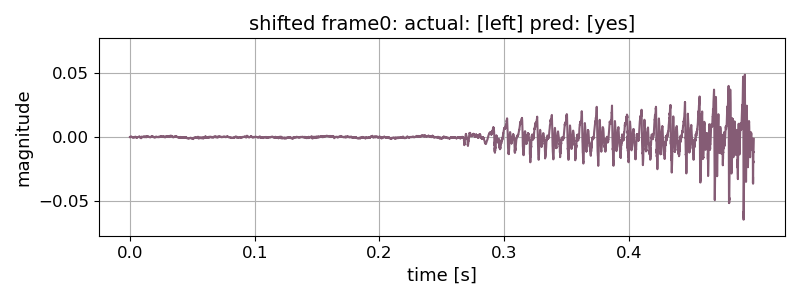
\includegraphics[width=0.48\textwidth]{./5_exp/figs/exp_details_tb_shift_left_frame0.png}}
    \quad
    \subfigure[frame shift 30]{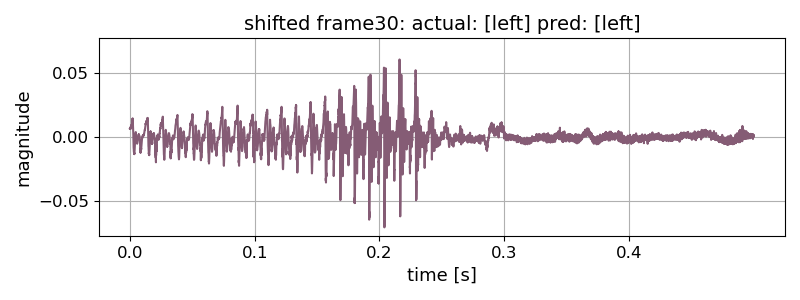
\includegraphics[width=0.48\textwidth]{./5_exp/figs/exp_details_tb_shift_left_frame30.png}}
    \subfigure[frame shift 59]{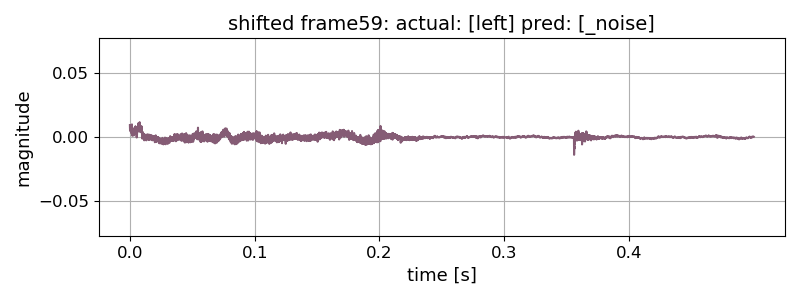
\includegraphics[width=0.48\textwidth]{./5_exp/figs/exp_details_tb_shift_left_frame59.png}}
  \caption{Shifting a self recorded example of the label \enquote{left} with certain amounts of frame shifts. The classification results are provided in the title annotations.}
  \label{fig:exp_details_tb_shift_left}
\end{figure}
\FloatBarrier
\noindent
The figures in this section present a correct classification with a colored pixel and an incorrect with a white pixel.
\rfig{exp_details_tb_shift} provides one example of a shift invariance test.
\begin{figure}[!ht]
  \centering
    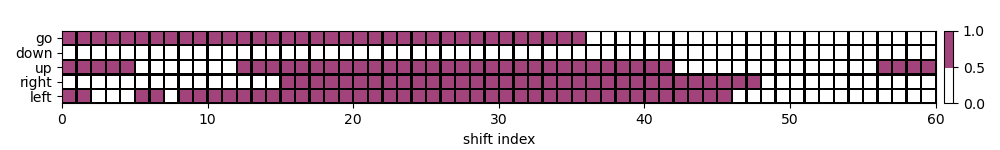
\includegraphics[width=0.65\textwidth]{./5_exp/figs/exp_fs_cepstral_tb_shift_conv-jim_mfcc12_norm0.png}
  \caption{Shift invariance test example selected from one of the trained models in the experiments.}
  \label{fig:exp_details_tb_shift}
\end{figure}
\FloatBarrier
\noindent
The purpose of the shift invariance test is not to achieve a full classification score upon each test example because this is hardly possible when not all of a keyword's information is captured within the shifted frame.
But to analyze whether there are consecutive correct classifications within a certain region on the shift index.
Holes in this region are not a good indicator for the trained model.
If one example could not be classified at all it does not necessarily imply that the trained model performs poorly but that this special example is not recognized with this specific model.
A well performing model usually has a wide region of correct classifications with no holes in it.


% --
% noise invariance

\subsubsection{Noise Invariance}
The classification of speech signals often requires noise invariance because a significant amount of noise usually is added from the use of poor microphones or recording set-ups and therefore might disturb the classification accuracy.
To construct a test upon noise invariance, AWGN is added to the test signal $\bm{x} \in \R^n$ by
\begin{equation}
  \bm{\tilde{x}} = \bm{x} + \bm{v}, \quad \bm{v} \sim \mathcal{N}(\mu, \sigma),
\end{equation}
where $\bm{v} \in \R^n$ is the additive normal noise sampled from $\mathcal{N}(\mu, \sigma)$ with mean $\mu = 0$ and standard deviation $\sigma$.
The AWGN is parametrized by the standard deviation $\sigma$ to create a certain Signal to Noise Ratio (SNR), denoted as $S$.
Rewriting the formula of the SNR, the standard deviation can be obtained by
\begin{equation}
  \sigma = \sqrt{\frac{\frac{1}{n}\bm{x}^T \bm{x}}{10^{\frac{S}{10}}}}
\end{equation}
for requested SNR values $S$ in decibel (dB).
A SNR level of zero means that there is equal energy of the added noise $\bm{v}$ and the test signal $\bm{x}$, therefore, the resulting signal is already strong disturbed with noise.
\rfig{exp_details_tb_noise_left} provides an example of the noise invariance test with a low, middle, and high SNR value.
\begin{figure}[!ht]
  \centering
    \subfigure[\SI{16}{\dB}]{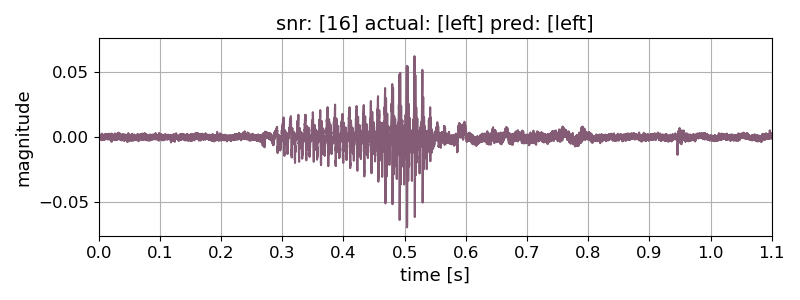
\includegraphics[width=0.48\textwidth]{./5_exp/figs/exp_details_tb_noise_left_snr16.png}}
    \quad
    \subfigure[\SI{0}{\dB}]{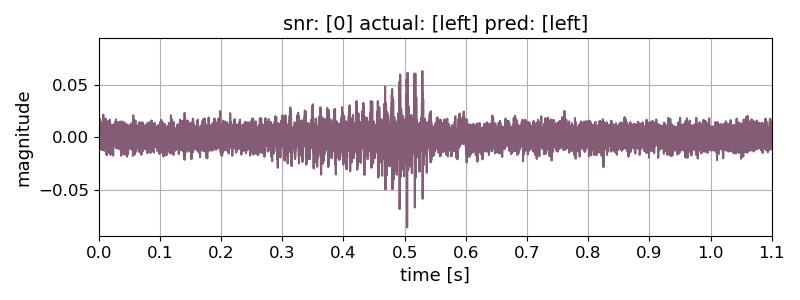
\includegraphics[width=0.48\textwidth]{./5_exp/figs/exp_details_tb_noise_left_snr0.png}}
    \subfigure[\SI{-16}{\dB}]{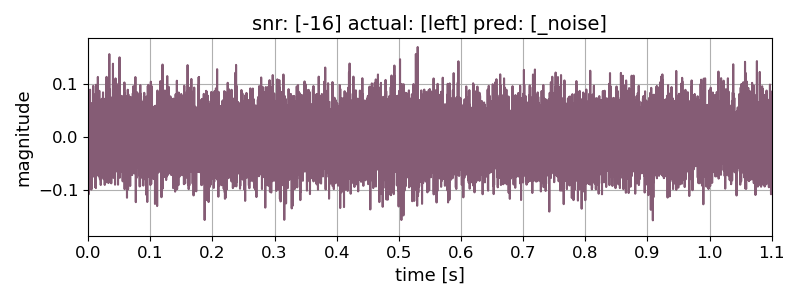
\includegraphics[width=0.48\textwidth]{./5_exp/figs/exp_details_tb_noise_left_snr-16.png}}
  \caption{Adding noise to a self recorded example of \enquote{left} with certain SNR values. The classification results are provided in the title annotations.}
  \label{fig:exp_details_tb_noise_left}
\end{figure}
\FloatBarrier
\noindent
The plots for the noise invariance indicate the added noise by the SNR value on the x-axis.
\rfig{exp_details_tb_noise} shows an example of a noise invariance test.
\begin{figure}[!ht]
  \centering
    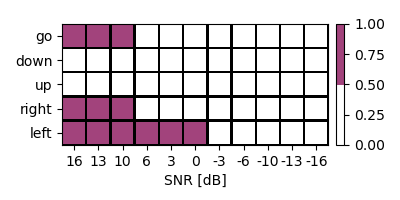
\includegraphics[width=0.35\textwidth]{./5_exp/figs/exp_fs_cepstral_tb_noise_conv-jim_mfcc12_norm0.png}
  \caption{Noise invariance test example selected from the trained models in the experiments.}
  \label{fig:exp_details_tb_noise}
\end{figure}
\FloatBarrier
\noindent
The same criteria, as described in the shift invariance, also applies to the noise invariance, where the region of consecutive correct classifications should start from low noise levels to high noise levels.